\section{Algorithm implementation}
\label{sec:algorithm_implementation}

In this section, we present the implementation of the three algorithms we are going to analyze in this report.
The algorithms are implemented in \texttt{MATLAB} and are designed to handle multiple dimensions problems, meaning that they can be used for both N-D environments.
In the following only the core of each algorithm is presented, leaving the code of all the auxiliaries classes such as \texttt{Graph}, \texttt{Edge}, or \texttt{Node} among the files in the repository.


\subsection{RRT algorithm}
\label{subsec:rrt_algorithm}

The most basic version of the single-query sampling-based algorithm is the Rapidly-exploring Random Tree (RRT) algorithm.
The RRT algorithm is nothing more than the direct implementation of the core algorithm presented in Figure \ref{fig:sampling_based_flowchart}.

Listing \ref{lst:rrt_algorithm} shows a possible implementation of the RRT algorithm.

\lstinputlisting[
    style=Matlab-editor,
    caption={Node class used to represent a node in the graph.},
    label={lst:rrt_algorithm}
]{files/rrt.m}


The algorithm takes as input the graph $G$, the map $M$, the start node $s$, and the goal node $g$.
It starts by initializing the tree $T$ with the start node and enters a loop where at first a random point/configuration is sampled from the workspace.
Then, it finds the nearest node already in the tree and generates a new node by moving in the direction of the sampled point.
If the new node is in collision with the obstacles, it's discarded and the algorithm skips to the next iteration.
If the new node is valid, it's added to the tree.
A final step is to check if the new node is close enough to the goal node, in which case the algorithm terminates and returns the path from the start node to the goal node, otherwise the algorithm continues to sample new points until a maximum number of iterations is reached, or the goal node is reached.

The RRT algorithm is simple and efficient, but lacks optimality in the generated path which is normally jagged and not smooth.
The algorithm is also not complete, meaning that it may not find a solution even if one exists in the configuration space due to the maximum number of iterations limit.
However, it has been proved that the RRT algorithm is probabilistically complete, meaning that as the number of iterations increases, the probability of finding a solution approaches 1 (at the cost of longer computation time, of course).



\subsection{RRT* algorithm}
\label{subsec:rrt_star_algorithm}

RRT* is an extension of the RRT algorithm that improves the optimality of the solution by rewiring the tree to find shorter paths.
The main idea behind the RRT* algorithm is to keep track of the cost of reaching each node in the tree and to rewire the tree whenever a new node is added.
This is done by checking if the new node can be used as a cheaper parent connection for any of the existing nodes in the tree.

Listing \ref{lst:rrt_star_algorithm} shows a possible implementation of the RRT* algorithm.

\lstinputlisting[
    style=Matlab-editor,
    caption={Code for the implementation of RRT* algorithm.},
    label={lst:rrt_star_algorithm}
]{files/rrtStar.m}


Again, the core structure of the algorithm is similar to the RRT algorithm, but with a few extra steps.
The algorithm starts by initializing the tree $T$ with the start node and enters a loop where it samples a random point in the configuration space.
Then, it finds the nearest node in the tree and generates a new node by moving towards the sampled point.
If the new node is in collision with the obstacles, it is discarded and the algorithm continues to sample a new point.
If the new node is valid, the algorithm at first connect it to the nearest node in the tree, and then checks if any of its neighbors can also be connected to it with a lower cost-to-go.
This analysis, called rewiring, help to construct a more optimal tree with smoother connections and consequently shorter paths.
Figure \ref{fig:rrt_star} shows an example of the rewiring process.

\begin{figure}[H]
    \centering
    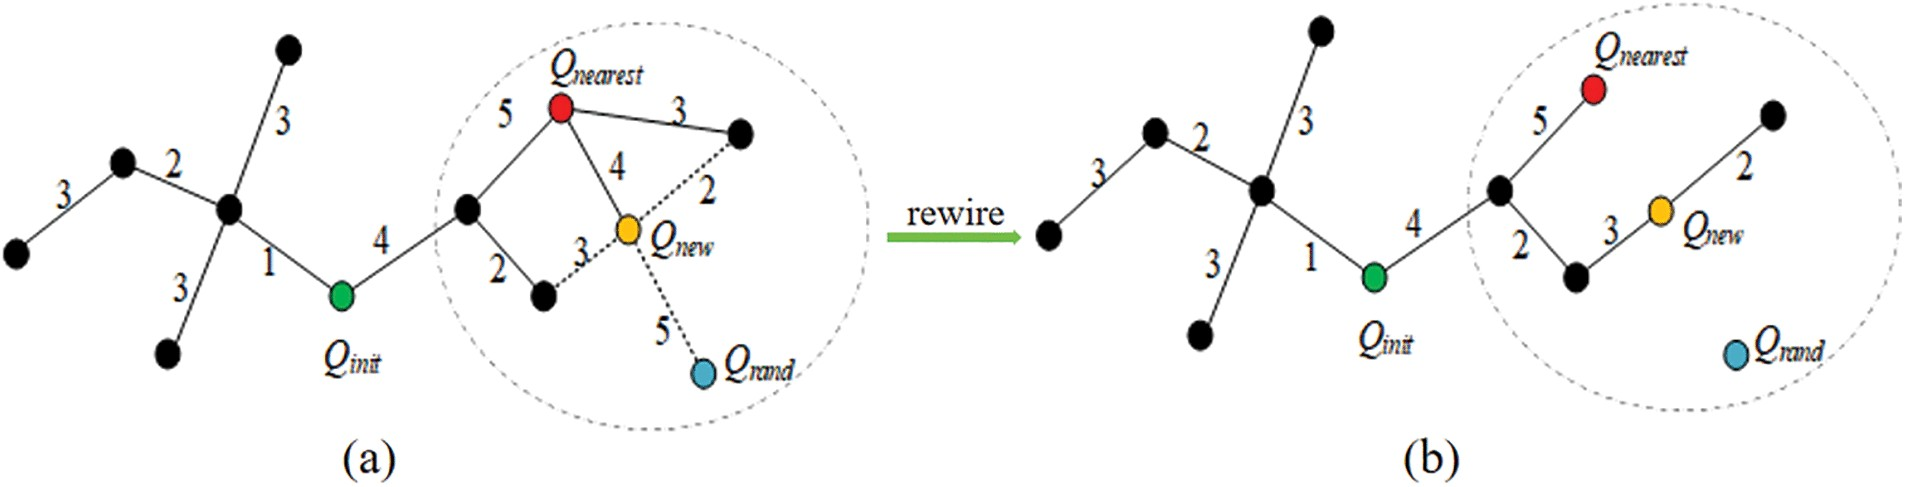
\includegraphics[width=1.0\textwidth]{./img/rrt_star.png}
    \caption{Example of the rewiring process in RRT* algorithm. Credit to \cite{JIANG20244303}.}
    \label{fig:rrt_star}
\end{figure}

As it is going to be shown in the next section, the RRT* algorithm is more efficient than the RRT algorithm in terms of path length, at the cost negligible increase in computation time.

\paragraph{Optimality convergence of RRT*}

As a final note, we recall that thanks to \cite{rrt_optimality}, it has been proved that the RRT* algorithm converges to the optimal solution as the number of sampled points goes to infinity and the rewiring radius is dynamically adjusted as:

\begin{equation}
    r_n = \gamma \left( \frac{\log{n}}{n} \right) ^ {\frac{1}{d+1}}
\end{equation}

Where $n$ is the number of sampled points, $d$ is the dimension of the configuration space, and $\gamma$ is a constant that depends on $d$.

Line 50 of the code in Listing \ref{lst:rrt_star_algorithm} shows a possible implementation of this dynamic rewiring radius.



\subsection{RRT-kinematic algorithm}
\label{subsec:rrt_kinematic_algorithm}

Finally, we move to the last algorithm we are going to implement, which is the RRT-kinematic algorithm.
The RRT-kinematic algorithm is a variant of the RRT algorithm that takes into account the kinematic constraints of the robot during the planning process.
This is particularly useful for vehicles with non-holonomic constraints, such as terrestrial vehicles or mobile robots.

Listing \ref{lst:rrt_kinematic_algorithm} shows a possible implementation of the RRT-kinematic algorithm.

\lstinputlisting[
    style=Matlab-editor,
    caption={Code for the implementation of RRT-kinematic algorithm.},
    label={lst:rrt_kinematic_algorithm}
]{files/rrtKinematic.m}

Again, we recognize the same core structure of the RRT algorithm, but with a few extra steps.
In particular, the choice of the new node is not done by simply moving towards the sampled point, but rather by generating a trajectory from the nearest node in the tree to the sampled point leveraging the kinematic model of the robot.
In the specific case of the implemented algorithm, we consider dealing with a \textit{Bicycle} model, which is a common model used to represent the motion of a car-like vehicle.
Starting from the nearest node in the tree, a random control input is sampled and a trajectory is generated by integrating the kinematic model of the robot over a fixed time horizon.
Collision checking is then performed and among all the tested trajectories, the one that is valid and has the lowest cost is selected as the new node to be added to the tree.
By doing so, we are sure that the generated path is feasible by the robot, respecting its kinematic constraints.

\paragraph{Bicycle kinematic model}

Even if the kinematic model of the vehicle is not the main focus of this report, we briefly present it here for completeness.
The kinematic model of the vehicle is described by the following equations:

\begin{figure}[H]

    \begin{minipage}{0.30\textwidth}

        \begin{equation}
            \begin{aligned}
                \dot{x}      & = v \cdot \cos(\theta)           \\
                \dot{y}      & = v \cdot \sin(\theta)           \\
                \dot{\theta} & = \frac{v}{L} \cdot \tan(\delta)
            \end{aligned}
        \end{equation}

    \end{minipage}
    %
    \hfill
    %
    \begin{minipage}{0.50\textwidth}

        \centering
        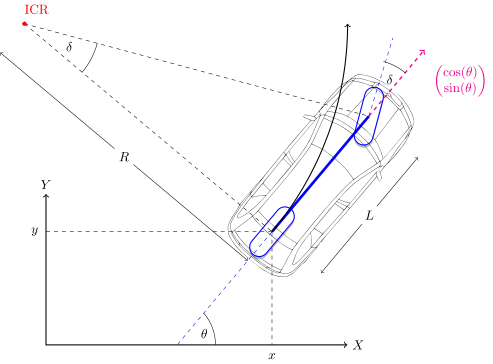
\includegraphics[width=1.0\textwidth]{./img/bicycle_model.png}

    \end{minipage}

    \caption{Bicycle kinematic model. Image credit to \href{https://thomasfermi.github.io/Algorithms-for-Automated-Driving/Control/BicycleModel.html}{Thomas Fermi}.}
    \label{fig:bicycle_model}

\end{figure}

Where $x$ and $y$ are the position of the vehicle in the workspace, $\theta$ is the heading angle of the vehicle, $v$ is the linear velocity, $L$ is the wheelbase of the vehicle (distance between the front and rear axles), and $\delta$ is the steering angle.

One can clearly see that the kinematic model is composed by a set of differential equations.
In order to simulate in time based on the control inputs and current state of the vehicle, we need to integrate these equations.
Different integration methods can be used, such as Euler integration or Runge-Kutta integration.
However, given the simplicity and expected slow dynamics of the model, we can use a simple Euler integration with a fixed time step $\Delta t$.

Listing \ref{lst:vehicle_model} shows a possible implementation of the kinematic model of the vehicle.

\lstinputlisting[
    style=Matlab-editor,
    caption={Code for the kinematic model of the vehicle.},
    label={lst:vehicle_model}
]{files/modelBicycle.m}
